\appendixsection{Артефакты наблюдаемости и метрик качества}
\label{app:observability}

В данном приложении приведены графические артефакты метрик, использованные в
работе как подтверждение наблюдаемости системы. Они не являются самостоятельным
доказательством промышленной производительности, а служат визуальным свидетельством
того, что ключевые стадии пайплайна --- gRPC-вызовы, публикация в Kafka и
обработка listener-ами --- действительно измеряются и сопоставимы между собой.

\begin{figure}[p]
    \centering
    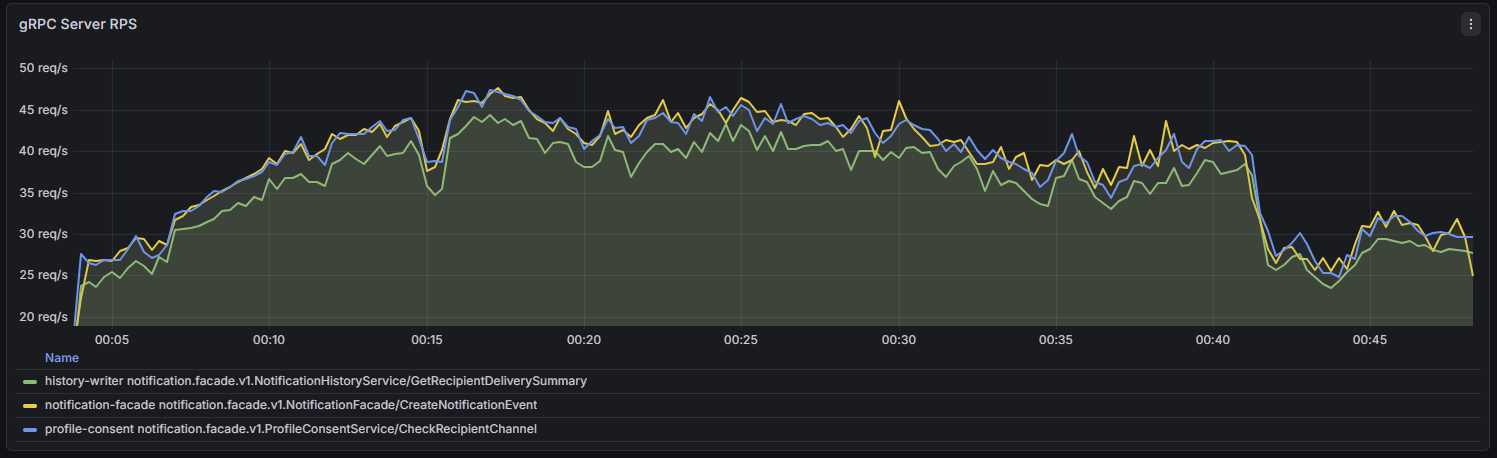
\includegraphics[width=\textwidth]{inc/server_rps.png}
    \caption{Интенсивность серверных gRPC-вызовов в ходе стендового прогона}
    \label{fig:appendix-server-rps}
\end{figure}

\begin{figure}[p]
    \centering
    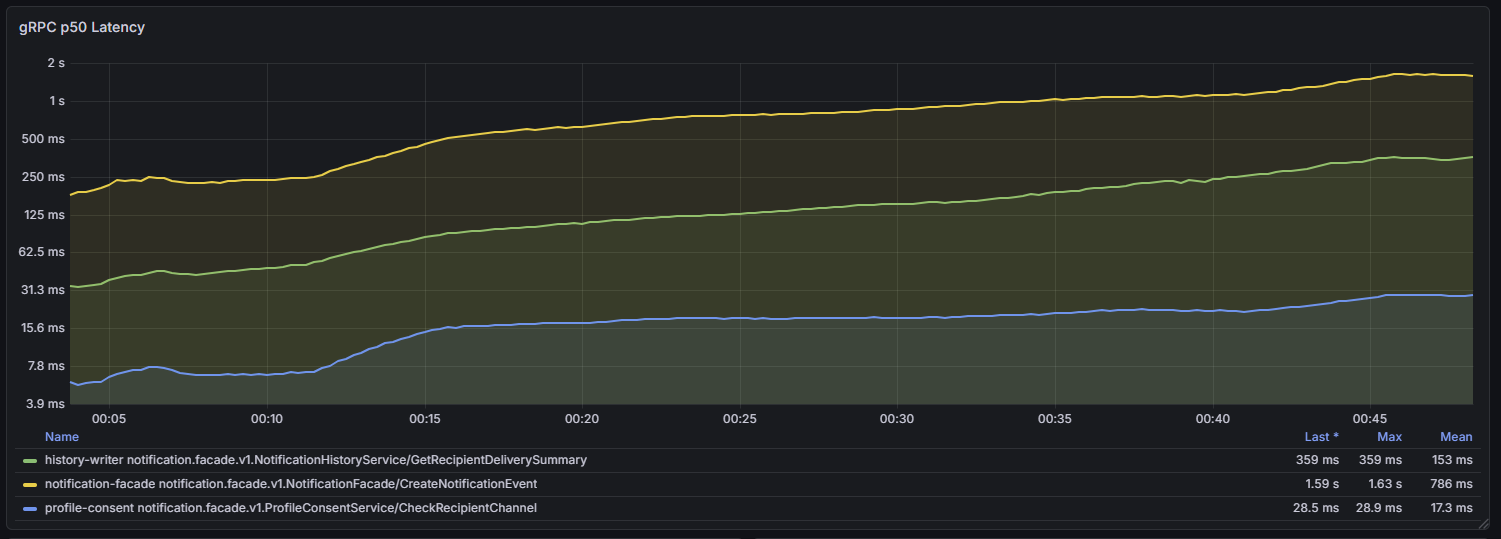
\includegraphics[width=\textwidth]{inc/grpc_p50_lat.png}
    \caption{Медианная задержка ключевых gRPC-вызовов}
    \label{fig:appendix-grpc-p50}
\end{figure}

\begin{figure}[p]
    \centering
    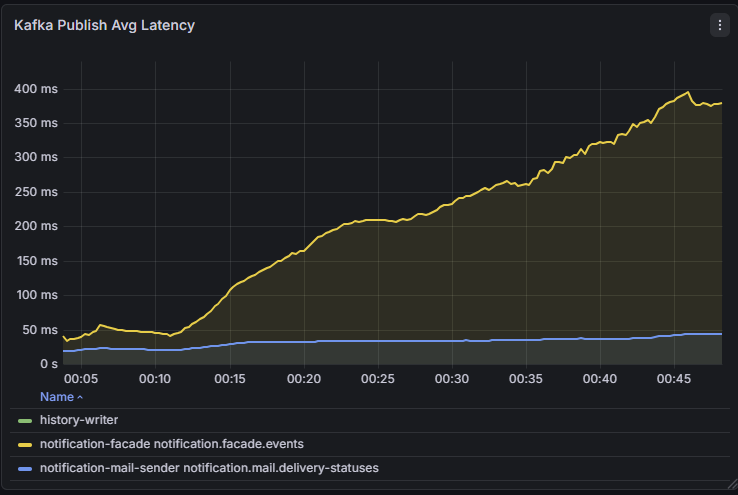
\includegraphics[width=\textwidth]{inc/kafka_avg_latency.png}
    \caption{Средняя задержка публикации сообщений в Kafka}
    \label{fig:appendix-kafka-publish-latency}
\end{figure}

\begin{figure}[p]
    \centering
    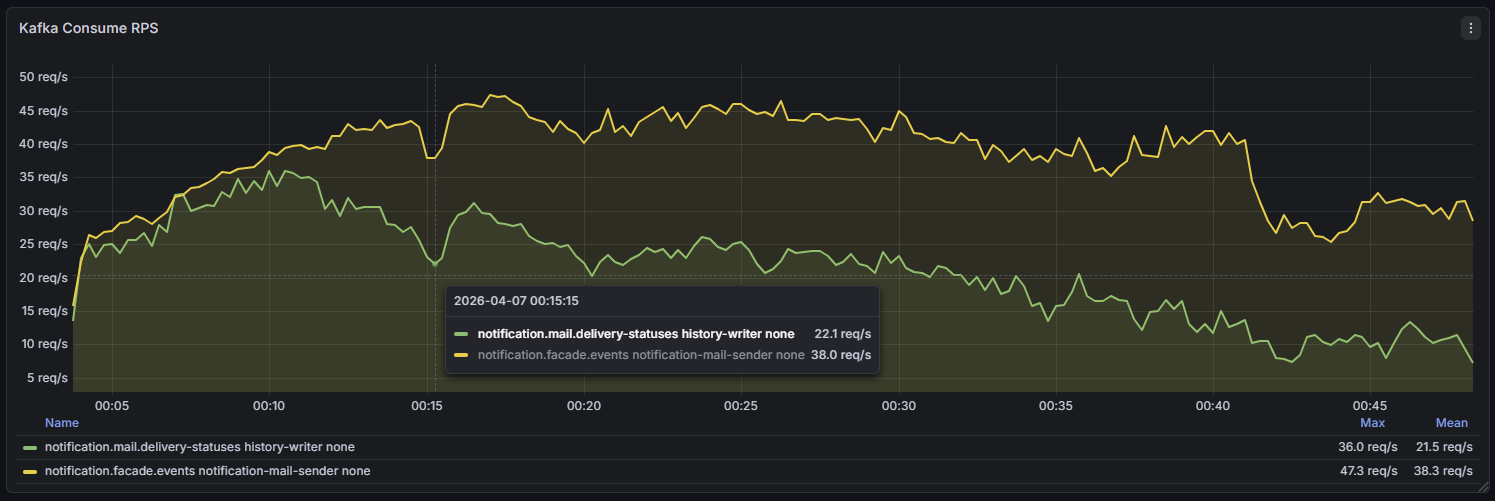
\includegraphics[width=\textwidth]{inc/kafka_consume_rps.png}
    \caption{Интенсивность потребления Kafka-сообщений на основных потребителях}
    \label{fig:appendix-kafka-consume-rps}
\end{figure}

\clearpage

Интерпретация приведённых артефактов выполняется в основной главе о тестировании.
В рамках приложения они сохраняются как подтверждение того, что:
\begin{enumerate}
    \item входные gRPC-вызовы фасада и профильного сервиса наблюдаемы по интенсивности и задержке;
    \item producer-операции Kafka отражаются в метриках времени публикации;
    \item consumer-операции sender-сервисов и history-сервиса наблюдаемы как по RPS, так и по времени обработки;
    \item метрики пригодны для сопоставления стадий одного и того же потока данных.
\end{enumerate}
